%\chapter{Pentesting}\label{ch:testing}
%\lstset{style=inline}
%
%This chapter describes the pentesting of the Wi-Fi environments, established with the RCSL.
%It starts by explaining some common (Wi-Fi-) network attacks, of which the cracking of WEP and WPA/WPA2 are then tested on the RCSL and the results documented.
%
%\section{Attacks}
%Wi-Fi attacks can take many different forms, depending on the type of attack and which mechanism it tries to break.
%There are attacks aimed at breaking the Access Controls, Integrity Controls, Confidentiality or Availability. \cite{Oriyano_2017}
%The following selection of attacks quite nicely depicts the different vectors an attacker can take to hack a Wi-Fi network and its STAs.
%
%\subsection{War Driving}
%War Driving describes the act of gathering information on Wi-Fi networks in larger numbers in order to locate specific or weak targets.
%This is done by traversing areas of interest with data collection equipment, which collects information about every network coming into range.
%After capturing and mapping as many Wi-Fi networks as possible, a more sophisticated attack can be launched on the captured networks, or the data can be sold on the black market. \cite{Oriyano_2017}
%
%\subsection{Rogue Access Point and Evil Twin}
%When using Rogue Access Points, attackers place extra APs onto a network, trying to stay undetected and get STAs to connect to the malicious AP.
%This can, for example, be done by connecting an AP to an open and unprotected LAN port inside a public or company building.
%Once a STA has connected to the rogue AP, it acts as a MitM, allowing the attacker to manipulate or eavesdrop on the traffic.
%
%Evil Twins have some similarity to Rogue Access Points in that they also pretend to be a legitimate part of an existing network.
%Different to Rogue APs, Evil Twins do not connect to the legitimate network, but instead spoof wireless networks, providing a stronger signal, to again get STAs to connect to it.
%Some attackers might also use a deauthentication flood to get STA disconnected from their genuine AP and auto connect to the malicious one.
%
%Because they employ one-way authentication, WEP and OWE networks are vulnerable to these attacks. \cite[page~105,119]{Sankaran_Gulasekaran_2021} 
%
%\subsection{Cracking WEP}
%As touched on in \cref{ch:basics_wifi}, WEP has several vulnerabilities, most notable the encryption algorithm, the one-sided authentication mechanism, and the lackluster MIC.
%
%WEP encryption is based on the RC4 algorithm and works "by exclusive-ORing the data stream with a pseudo-random stream of bits generated based on the WEP key" \cite[page~104]{Sankaran_Gulasekaran_2021} and a 24-bit initialization vector (IV).
%With 24 bits, there are about 16.5 million combinations for the IV, which can be exhausted in a few hours of network traffic.
%The probability of the same key being reused is at about 50\% after around 5000 frames have been captured, opening the possibility for reverse engineering by analysis of the frames \cite{Oriyano_2017}.
%%Because of this weak encryption mechanism, the password can be reverse engineered by analysing the frames and creating a decryption table.
%
%The MIC with CRC-32 is not sufficient in ensuring message integrity, allowing manipulated frames, injected into the network, to be accepted as non-compromised. \cite{Oriyano_2017}
%
%
%Cracking a WEP network involves the reverse engineering of the password, aided by exploiting the authentication mechanism and the MIC.
%The process begins by scouting the target network, commonly conducted by capturing all traffic on all channels from networks in the vicinity.
%In normal operation, a NIC only receives the traffic addressed to its MAC address.
%To disable this filtering, the network card is put into monitor mode, allowing it to capture all packets transmitted in the vicinity, and discover all APs present.
%After the target network has been determined, its traffic is captured, and after enough frames have been transmitted, the password can be reverse engineered.
%
%However, the process can be accelerated by injecting spoofed ARP frames to artificially increase traffic.
%This technique is called a replay attack and involves the capture of several authentic ARP frames, subsequently modifying and injecting them, which "the AP will re-broadcast [...] and as a result generate [new IVs]" \cite{Oriyano_2017}.
%
%Sending ARP frames without association to the AP will lead to them being rejected, therefore another spoofed frame is injected to fake authentication and association with the AP.
%
%\subsection{Cracking WPA/WPA2}
%WPA and WPA2 networks come with improved encryption in the form of TKIP and SAE-CCMP, which cannot be cracked in the way, WEP can \cite{Oriyano_2017}.
%To crack a WPA network, it is common to attack the authentication mechanism because, as described in \cref{ch:basics_wifi}, it can be vulnerable to offline attacks.
%
%An attacker starts off by capturing the handshake between an AP and STA during authentication, from which the PSK is extracted.
%In order to capture a handshake, the attacker would have to wait for a device to authenticate with the network, which depending on the number of STAs, could take quite some time.
%A deauthentication attack is performed, injecting frames, which force the STAs to reconnect to the AP and therefore making the capture of a handshake predictable.
%
%Since the PSK is derived from the password and other information, which is openly available, the password can be brute forced by generating PSKs and comparing them to the captured one.
%The brute force attack can be accelerated by performing a dictionary attack.
%However if the network uses a strong password, which is not contained in the password dictionary, the attack will be unsuccessful in the way that it takes too long to brute force the passphrase.
%Furthermore, APs with PMF enabled can not be attacked with this method, since encrypted deauthentication frames cannot be spoofed.
%
%\section{Methods}\label{sec:testing_methods}
%The pentests were conducted using the Aircrack-ng suite with Kali Linux.
%Kali Linux is a Linux distribution, which comes with a vast collection of tools for pentesting, security auditing and computer forensics.
%The Aircrack-ng suite is tailored towards network security assessment and is included with Kali Linux.
%\\\textit{Note: For more information, consult the Kali and Aircrack-ng documentation \cite{aircrack_ng}\cite{kali_docs}.}
%
%\begin{figure}[h]
%    \centering
%    \includegraphics[width=0.9\linewidth]{figures/Abbildungen/attack_setup.pdf}
%    \caption{illustration of the test setup}
%    \label{fig:test_setup}
%\end{figure}
%
%All tests were run on a Dell Vostro 3550 with an Intel Core i3 CPU from 2011 and 8GB of RAM, using the Alfa AWUS036AXM network card.
%
%\subsection{Cracking WEP}{\label{ssec:method_WEP}}
%The RSCL is used to establish a WEP network to be cracked (see \cref{fig:test_setup}).
%Starting the target scouting, \lstinline[]|airmon-ng start wlan1| is used, which puts the card into monitor mode and creates a new network interface, called "wlan1mon".
%With the card being able to sniff all traffic in the area, the target network can be searched by using \lstinline[]|airodump-ng wlan1mon|.
%
%\begin{figure}[h]
%    \centering
%    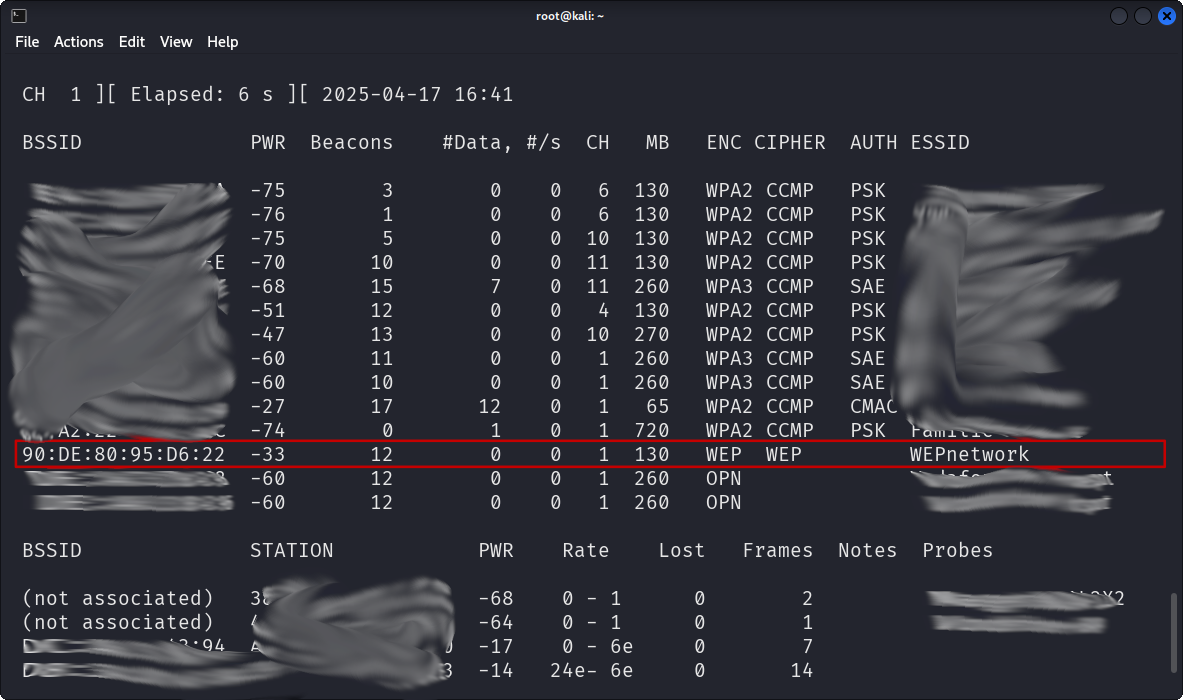
\includegraphics[width=\textwidth]{figures/Abbildungen/Screenshots/airodump_WEP.png}
%    \caption{Screenshot of airodump-ng}
%    \label{fig:airodump-ng}
%\end{figure}
%
%As seen in \cref{fig:airodump-ng}, the program scans on all channels for networks within reach and lists them in the table on top.
%The target network, marked with the red border, is listed with its respective BSSID, RSSI, recorded Beacon Frames, encryption standard, and cipher.
%
%In the second table, all STAs in reach are listed and to which AP they are associated.
%If a STA is actively scanning for networks, it is also listed with the network name it is probing for.
%
%%After the target network has been identified, airodump-ng is set up with filters to capture all traffic related to the AP and write it into a file with:
%%\lstinline[]|airodump-ng --channel 9 --bssid 00:28:6C:E4:40:80 --write CrackWEP wlan1mon|
%After the target network has been identified, airodump-ng is set up with filters to capture all traffic related to the AP and write it into an output file as seen in \cref{fig:airodump-ng_target}.
%
%\begin{figure}[h]
%    \centering
%    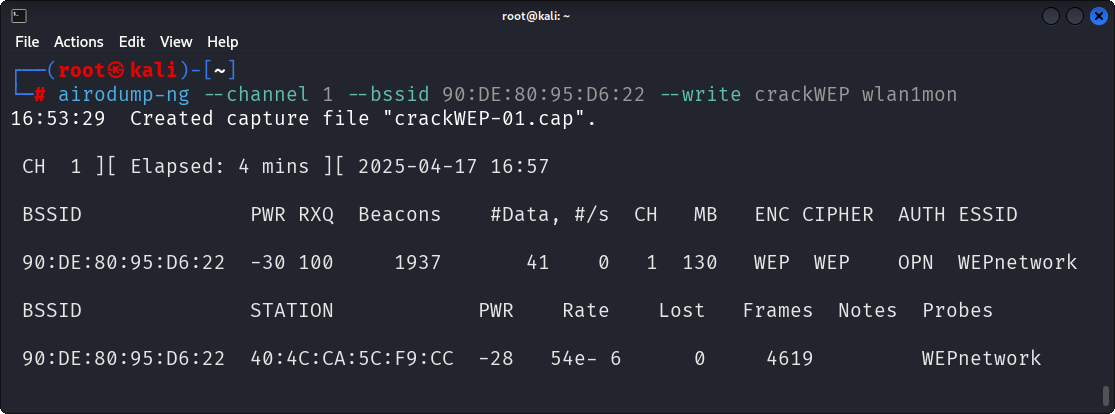
\includegraphics[width=\textwidth]{figures/Abbildungen/Screenshots/airodump_WEPcrack.png}
%    \caption{Screenshot of airodump-ng filtered for the target network}
%    \label{fig:airodump-ng_target}
%\end{figure}
%
%\lstinline[]|--channel| filters the captured frames to only collect frames on the APs channel 
%\\\lstinline[]|--bssid| filters the frames related to the BSSID of the target 
%\\\lstinline[]|--write| specifies the output file
%\\All devices associated with the network can be seen in the lower table, which at that time is only the ESP32 with the address \lstinline[]|40:4C:CA:5C:F9:CC|.
%
%For the replay attack, a fake association with the AP is established, using \lstinline[]|aireplay-ng| as seen in \cref{fig:aireplay-ng}. 
%\\\lstinline[]|--fakeauth 0| defines the authentication to be performed infinitely until a connection is established. 
%\\\lstinline[]|-e| sets the name of the target network
%\\\lstinline[]|-a| sets the BSSID of the target network
%\\\lstinline[]|-h| sets the MAC of the device to be associated with the target network
%
%\begin{figure}[h]
%    \centering
%    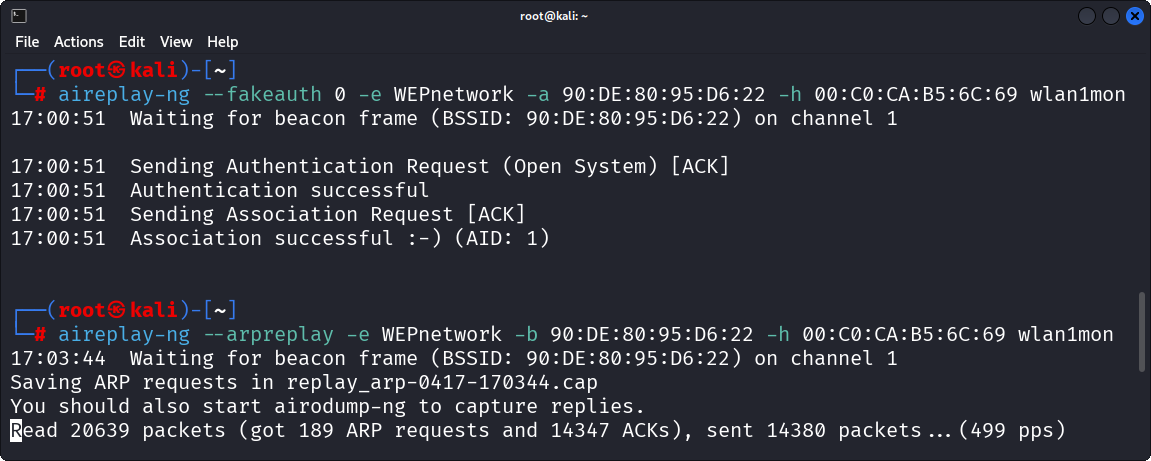
\includegraphics[width=\textwidth]{figures/Abbildungen/Screenshots/aireplay.png}
%    \caption{Screenshot of aireplay-ng fake authentication and ARP replay attack}
%    \label{fig:aireplay-ng}
%\end{figure}
%
%Upon successful association, as seen in \cref{fig:aireplay-ng}, ARP requests can be injected.
%\\\lstinline[]|--arpreplay| selects the replay attack for ARP frames
%\\\lstinline[]|-b| sets the BSSID of the target network
%\\\lstinline[]|-h| sets the MAC address of the attacker
%
%Creating and capturing traffic, IVs are collected, and the cracking of the password can be started simultaneously. 
%As seen in \cref{fig:aircrack-ng_WEP_process}, \lstinline[]|aircrack-ng| is executed and reads the output of airodump-ng, attempting to crack the password for every 5000 IVs collected.
%
%\begin{figure}[h]
%    \centering
%    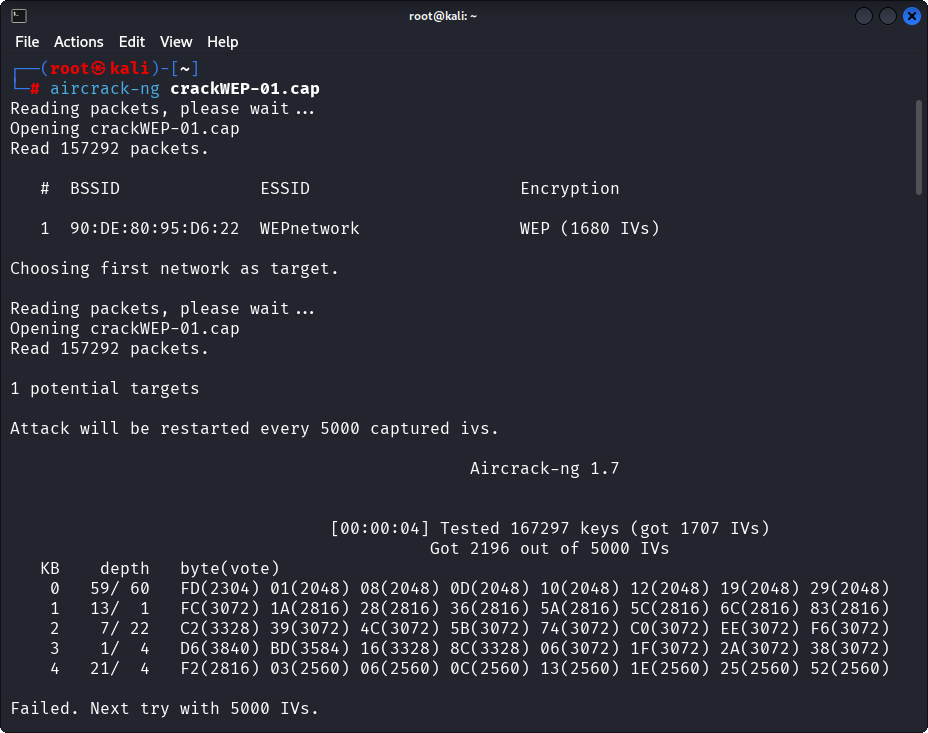
\includegraphics[width=\textwidth]{figures/Abbildungen/Screenshots/aircrack_WEP_03_01.png}
%    \caption{Screenshot of the cracking process with aircrack-ng}
%    \label{fig:aircrack-ng_WEP_process}
%\end{figure}
%
%\newpage
%\subsection{Cracking WPA/WPA2}
%This attack starts off by scouting the target network with \lstinline[]|airodump-ng| as well, in this case it is called "WPAnetwork".
%
%Once the desired AP has been discovered, \lstinline[]|airodump-ng| is used to capture the (re-)authentication handshake.
%To ensure the functionality of frame injection, it was tested with airodump, using the \lstinline[]|--test| flag.
%The output, depicted in \cref{fig:aireplay_test_WPA}, means that normal frames are ignored, due to the STA not being authenticated.
%If PMF is not active, deauthentication frames can still be injected.
%
%The deauthentication attack is performed with \lstinline[]|aireplay-ng| to force the re-authentication of connected STAs (see \cref{fig:aireplay_deauth}).
%
%\begin{figure}[h]
%    \centering
%    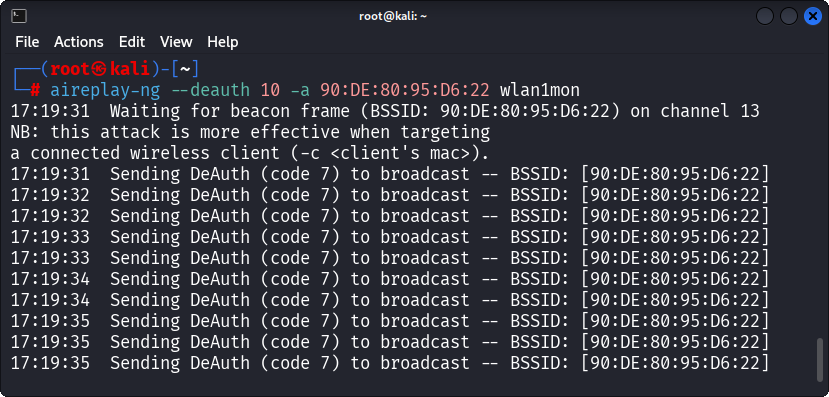
\includegraphics[width=\textwidth]{figures/Abbildungen/Screenshots/aireplay_deauth.png}
%    \caption{Screenshot of the Deauthentication Attack}
%    \label{fig:aireplay_deauth}
%\end{figure}
%
%\lstinline[]|--deauth 10| promts the program to transmit 10 deauthentication frames
%\\\lstinline[]|-a| specifies the APs BSSID, leading to the frames being broadcast to all STAs
%\\\lstinline[]|-c| can be used to specify the MAC address of a STA, to send the frames directly to a specific STA, as recommended by the program
%
%After capturing the authentication handshake, a dictionary attack is performed to crack the password, which in this case utilizes the "rockyou.txt" password list, built into Kali Linux, to brute force the password.
%
%Aircrack-ng starts to iterate through the password list, computes the PSK for each password and compares it to the captured PSK.
%The brute forcing is started with:
%\\\lstinline[]|aircrack-ng -b [BSSID] -w [passwordlist] WPAcrack-01.cap|
%
%\lstinline[]|-b| specifies the AP to be targeted
%\\\lstinline[]|-w| specifies the password file, in this case the rockyou.txt, found in \textit{/usr/share/wordlists}
%
%
%\section{Results}\label{sec:results}
%Navigation of the UI seems intuitive, and switching between menus works fluidly.
%Execution of the various scripts is reliable, if implemented correctly.
%However, the ESP32 has been observed to crash occasionally during Wi-Fi connection establishment.
%The circumstances and cause for the occurrence of these sporadic crashes are unclear at the moment, and a fix is not foreseen for the scope of this thesis.
%
%Upon conducting the tests, it was discovered that the configurations for the WEP, WPA and WPA2 networks were not correctly set up.
%The faulty configuration resulted in the network, supposedly encrypted with the WEP encryption standard, showing up as a WPA network in \lstinline[]|airodump-ng|.
%Also, the WPA and WPA2 networks were identified by airodump as WPA3 networks, using SAE as the authentication mechanism.
%The \cref{sec:network_management} details the process of resolving the configuration errors and allowing the following tests to be conducted.
%
%The webapp functions, specifically the MQTT communication and Juice Shop server, seem to work without complications, but were not tested thoroughly.
%
%\subsection{Cracking WEP}
%The first attempt at cracking the WEP network was unsuccessful because only the ESP32 being connected to the network, ARP request injection seemed unable to generate significant traffic, therefore the collection of IVs proceeds very slowly.
%
%As a workaround for test two, the RPI was connected to the internet and a second STA in form of a Smartphone was put on the network.
%The smartphone streamed a video, which generated sufficient traffic.
%This time, the password could be cracked after around three minutes and only 214 captured IVs.
%
%For control, a third test was conducted, for which the password of the hotspot was changed with the new password function.
%Again, the password could be cracked in about two minutes, with around 15000 IVs collected.
%
%\begin{figure}[h]
%    \centering
%    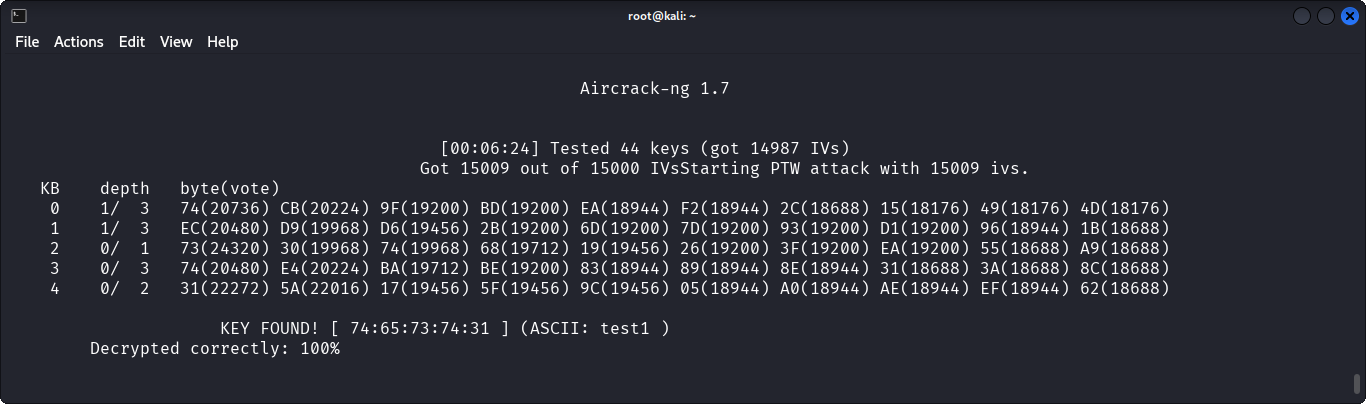
\includegraphics[width=\textwidth]{figures/Abbildungen/Screenshots/aircrack_WEP_03_03.png}
%    \caption{Screenshot of the fourth cracking attempt}
%    \label{fig:aircrack-ng_WEP_success}
%\end{figure}
%
%An investigation into the first test revealed that the ARP injection did not function properly, therefore a fourth test without the video stream was conducted.
%With working ARP injection, the IV collection proceeded quicker than in test one, however it still took around 20 minutes of frame capture and six minutes of cracking, as depicted in \cref{fig:aircrack-ng_WEP_success}, to find the password.
%
%\newpage
%\subsection{Cracking WPA/WPA2}
%On the first test, cracking the password was unsuccessful because the handshake was not captured, leading to aircrack-ng exiting with the output depicted in \cref{fig:aircrack-ng_WPA_handshake}.
%
%\begin{figure}[h]
%    \centering
%    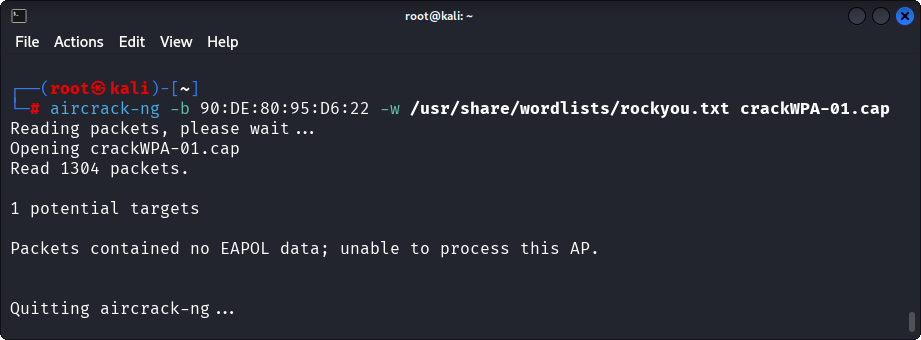
\includegraphics[width=\textwidth]{figures/Abbildungen/Screenshots/aircrack_WPA_01_01.png}
%    \caption{Screenshot of the failed handshake capture}
%    \label{fig:aircrack-ng_WPA_handshake}
%\end{figure}
%
%On the second try, a handshake was captured by manually reconnecting the EPS32 to the network.
%Capture of a handshake with the use of the deauthentication attack could not be achieved.
%With the password "TestSetup123", created on creation of the connection, the network could not be cracked with the RockYou password list.
%Since this password is not contained in the list, after two hours, the password could not be found, as to be seen in \cref{fig:aircrack-ng_WPA_fail}.
%
%After setting a new random password for the third try, cracking the network, shown in \cref{fig:aircrack-ng_WPA_success} was possible in 22 seconds.
%Multiple follow-up tries with other passwords also resulted in the successful cracking of the network, with the limitation of needing to manually (re-)connect the ESP32 to the network.
%
%Cause for the failing deauthentication attacks is most likely PMF being active for the network.
%Even though the configuration was double-checked, the previous unexpected behavior of Network Manager leads to the suspicion that the configuration is not being applied correctly.
%
%\begin{figure}[h]
%    \centering
%    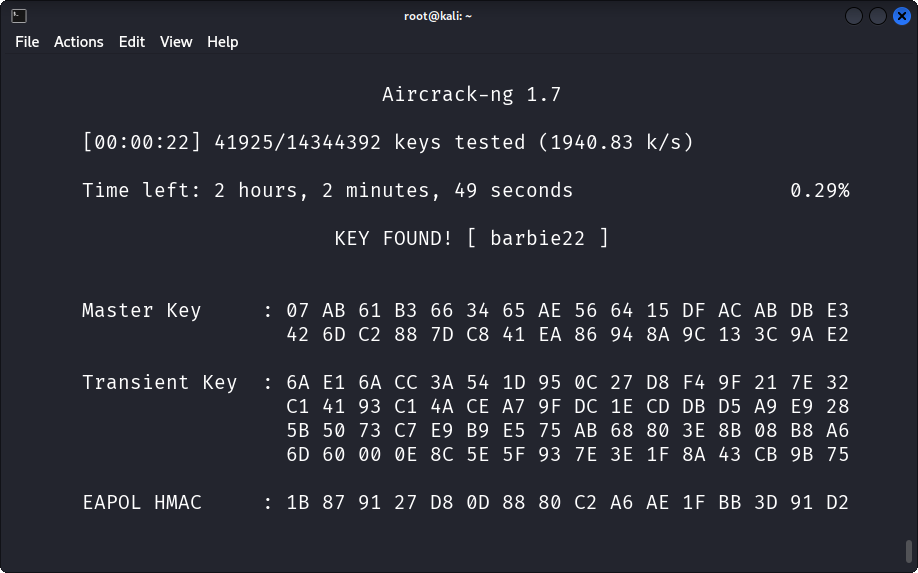
\includegraphics[width=\textwidth]{figures/Abbildungen/Screenshots/aircrack_WPA_success.png}
%    \caption{Screenshot of the successful cracking of WPA}
%    \label{fig:aircrack-ng_WPA_success}
%\end{figure}
%
{
\section{Pentesting Demonstration}

\begin{frame}
    \centering
    \tableofcontents[currentsection]
\end{frame}

\begin{frame}{Übersicht}
    \centering
    \includegraphics[width=.7\textwidth]{figures/attack_setup.pdf}
\end{frame}

\begin{frame}{Zusammenfassung}
    \fontsize{8}{8}\selectfont
    \begin{columns}
        \begin{column}{0.33\textwidth}
            %\begin{itemize}
            %    \item Sniffig aller Pakete mit Monitor Mode    
            %    \item Filter für Ziel AP
            %\end{itemize}
        \end{column}

        \begin{column}{0.33\textwidth}
            \begin{itemize}
                \item nötig für ARP Replay  
                \item möglich durch CRC32
            \end{itemize}
        \end{column}

        \begin{column}{0.33\textwidth}
            \begin{itemize}
                \item Injektion von ARP Paketen
                \item Erzeugen von IVs 
            \end{itemize}
        \end{column}
    \end{columns}

    \vspace{0.2cm}
    \begin{center}
        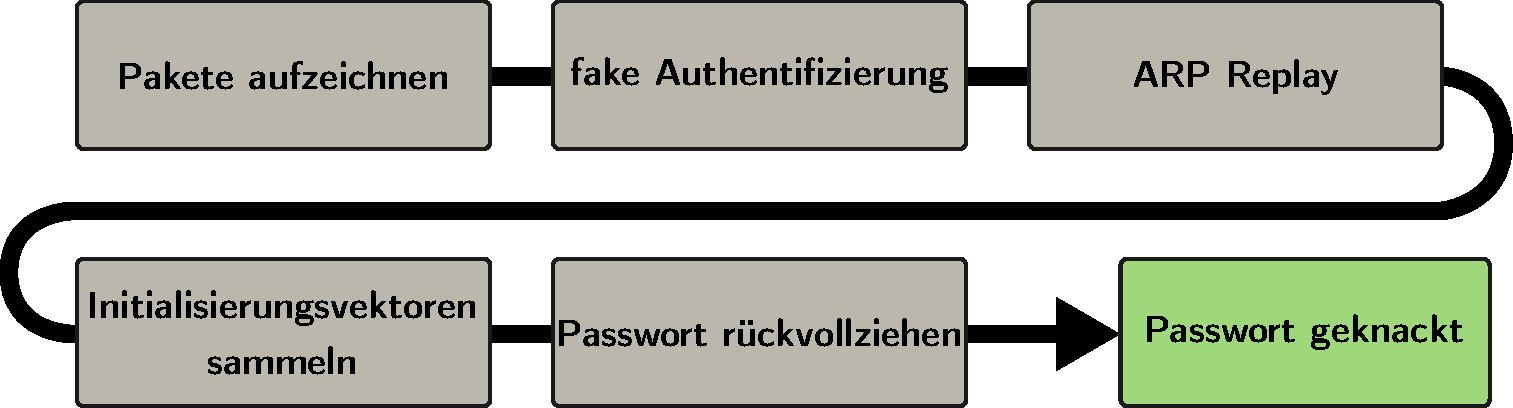
\includegraphics[width=0.9\textwidth]{figures/WEP_cracking.pdf}
    \end{center}

    \begin{columns}
        \begin{column}{0.33\textwidth}
           \begin{itemize}
                \item hohe Wahrscheinlickeit der Wiederholung
           \end{itemize} 
        \end{column}

        \begin{column}{0.33\textwidth}
           \begin{itemize}
                \item möglich bei Wiederholung der IVs
           \end{itemize} 
        \end{column}

        \begin{column}{0.33\textwidth}
            %\begin{itemize}
            %    \item Ausführung von folgenden Netzwerkangriffen möglich
            %\end{itemize}
        \end{column}

    \end{columns}
    \vspace{0.3cm}

\end{frame}
}